\documentclass[aspectratio=169,xcolor=table]{beamer}
\usepackage[utf8]{inputenc}
\usepackage[T1,T5]{fontenc}
\usepackage{amsmath,booktabs,array,graphicx,pifont,tikz}
\usetikzlibrary{arrows.meta,calc,positioning,fit,backgrounds}

\definecolor{Primary}{HTML}{111B88}
\definecolor{Secondary}{HTML}{101659}
\definecolor{Accent}{HTML}{F2A900}
\definecolor{SoftBlue}{HTML}{EAF2F8}
\definecolor{SoftGray}{HTML}{F3F5F7}
\definecolor{TextGray}{HTML}{4D5966}
\definecolor{RiskRed}{HTML}{A23B3B}
\definecolor{GoodGreen}{HTML}{26734D}
\mode<presentation>{\usetheme{Madrid}\usecolortheme{default}\setbeamertemplate{navigation symbols}{}}
\setbeamercolor{structure}{fg=Primary}
\setbeamercolor{frametitle}{fg=white,bg=Primary}
\setbeamercolor{title}{fg=white,bg=Primary}
\setbeamercolor{block title}{fg=white,bg=Primary}
\setbeamercolor{block body}{fg=black,bg=SoftBlue}
\setbeamercolor{block title alerted}{fg=white,bg=Accent!85!black}
\setbeamercolor{block body alerted}{fg=black,bg=Accent!12}
\setbeamercolor{section in head/foot}{fg=white,bg=Primary}
\setbeamercolor{author in head/foot}{fg=white,bg=Secondary}
\setbeamercolor{date in head/foot}{fg=white,bg=Primary}
\setbeamerfont{section in head/foot}{size=\tiny,series=\bfseries}
\setbeamerfont{author in head/foot}{size=\scriptsize}
\setbeamerfont{date in head/foot}{size=\scriptsize,series=\bfseries}
\setbeamerfont{frametitle}{series=\bfseries}
\setbeamerfont{title}{series=\bfseries}
\newcommand{\decklabel}{Catch-up 03/10/2026}
\setbeamertemplate{itemize item}{\color{Secondary}$\blacktriangleright$}
\setbeamertemplate{itemize subitem}{\color{Accent}$\bullet$}
\setbeamertemplate{headline}{\leavevmode\begin{beamercolorbox}[wd=\paperwidth,ht=2.7ex,dp=1.1ex,leftskip=.35cm,rightskip=.35cm]{section in head/foot}\insertsectionnavigationhorizontal{\dimexpr\paperwidth-.70cm\relax}{}{}\end{beamercolorbox}}
\setbeamertemplate{footline}{\leavevmode\hbox{\begin{beamercolorbox}[wd=.55\paperwidth,ht=2.6ex,dp=1ex,leftskip=.35cm,rightskip=.20cm]{section in head/foot}\usebeamerfont{section in head/foot}\insertsectionhead\end{beamercolorbox}\begin{beamercolorbox}[wd=.27\paperwidth,ht=2.6ex,dp=1ex,center]{author in head/foot}\usebeamerfont{author in head/foot}\decklabel\end{beamercolorbox}\begin{beamercolorbox}[wd=.18\paperwidth,ht=2.6ex,dp=1ex,rightskip=.35cm plus1fil]{date in head/foot}\usebeamerfont{date in head/foot}\hfill\insertframenumber\,/\,\inserttotalframenumber\end{beamercolorbox}}}

\newcommand{\hi}[1]{\textcolor{Primary}{\textbf{#1}}}
\newcommand{\bad}[1]{\textcolor{RiskRed}{\textbf{#1}}}
\newcommand{\good}[1]{\textcolor{GoodGreen}{\textbf{#1}}}
\newcommand{\src}[1]{{\tiny\color{TextGray}[Nguồn: #1]}}
\newcommand{\cmark}{\textcolor{GoodGreen}{\ding{51}}}
\newcommand{\xmark}{\textcolor{RiskRed}{\ding{55}}}
\newcommand{\pmark}{\textcolor{Accent!85!black}{\ding{108}}}
\tikzset{
  box/.style={draw=Primary,fill=SoftBlue,rounded corners=2pt,align=center,font=\small,minimum height=0.9cm},
  lgbox/.style={draw=Accent!85!black,fill=Accent!13,rounded corners=2pt,align=center,font=\small,minimum height=0.9cm},
  nbox/.style={draw=TextGray,fill=SoftGray,rounded corners=2pt,align=center,font=\small,minimum height=0.9cm},
  outbox/.style={draw=GoodGreen,fill=GoodGreen!10,rounded corners=2pt,align=center,font=\small\bfseries,minimum height=0.9cm},
  arr/.style={-{Latex[length=2mm]},thick,draw=TextGray},
}

\title{Contextual Biasing cho ASR:\\Benchmark \& Baseline}
\subtitle{Báo cáo tiến độ theo next step buổi họp 17/09 \textbullet\ Mục tiêu Interspeech 2027}
\author{Nhóm Contextual ASR}
\institute{}
\date{03/10/2026}
\setbeamertemplate{title page}{\begin{centering}\vspace*{0.10cm}
\includegraphics[height=1.08cm]{imgs/logo.png}\par\vspace{0.32cm}\begin{beamercolorbox}[sep=0.50em,center,rounded=true]{title}\usebeamerfont{title}\inserttitle\par\vspace{0.14cm}{\small\insertsubtitle\par}\end{beamercolorbox}\vspace{0.42cm}{\usebeamerfont{author}\insertauthor\par}\vspace{0.10cm}{\usebeamerfont{institute}\insertinstitute\par}\vfill{\usebeamerfont{date}\insertdate\par}\end{centering}}

\begin{document}
\begin{frame}[plain]\titlepage\end{frame}

% =====================================================================
\section{Tóm tắt}
\begin{frame}{Hôm nay em báo cáo 3 điều}
\begin{center}
\begin{tikzpicture}[node distance=0.35cm]
\node[box,minimum width=4.0cm,text width=3.8cm,minimum height=1.7cm] (a) {\textbf{1. Đã làm gì?}\\\footnotesize next step 17/09: benchmark, metric, chạy baseline};
\node[box,right=of a,minimum width=4.0cm,text width=3.8cm,minimum height=1.7cm] (b) {\textbf{2. Số nói gì?}\\\footnotesize số tin được không, gợi ra bài toán gì};
\node[lgbox,right=of b,minimum width=4.0cm,text width=3.8cm,minimum height=1.7cm] (c) {\textbf{3. Làm gì tiếp?}\\\footnotesize kế hoạch 2 tuần + cần thầy quyết};
\draw[arr] (a)--(b); \draw[arr] (b)--(c);
\end{tikzpicture}
\end{center}
\vspace{0.35cm}
\begin{beamercolorbox}[sep=0.6em,rounded=true]{block body alerted}
\small\textbf{Kết luận trước:}
\begin{itemize}\itemsep2pt
\item Benchmark + baseline \textbf{đã xong}, khớp số chính thức.
\item Qwen3-ASR frozen \textbf{dùng context rất tốt} nếu list \textbf{ngắn và có từ đúng} (B-WER $-46\%$); list dài hoặc sai thì \textbf{vô dụng, thậm chí hại}.
\item Các paper mạnh nhất đều giả định \textbf{list cho sẵn}. Em đề xuất bài toán \textbf{tự dựng list}, và xin 2 tuần làm \textbf{feasibility} trước khi chốt method.
\end{itemize}
\end{beamercolorbox}
\end{frame}

% =====================================================================
\section{1. Đã làm gì}
\begin{frame}{Next step buổi 17/09 $\rightarrow$ trạng thái}
\small\renewcommand{\arraystretch}{1.3}
\begin{tabular}{@{}p{3.6cm}p{8.6cm}c@{}}
\toprule
\textbf{Thầy giao} & \textbf{Đã làm} & \\
\midrule
Dựng benchmark dataset & LibriSpeech + bias list IS21 --- đúng bộ mà Hou25 và PTC-Bias dùng & \cmark\\
Dataset theo domain & Đề xuất \hi{ConEC} (earnings call, giọng thật, context thật); bộ thuhcsi là \bad{tiếng Trung} & \pmark\\
Metric & WER / U-WER / B-WER bằng \textbf{scorer chính thức}; Recall@K cho bước tạo list & \cmark\\
Chạy rồi ``xem'' & Qwen3-ASR $\times$ 7 điều kiện $\times$ 2 tập (5.559 câu, 1$\times$RTX 4090); Whisper tái hiện Hou25 & \cmark\\
Paper không code $\rightarrow$ tự làm & Đã đối chiếu setting 2 paper; PTC-Bias \textbf{có code}, Hou25 \textbf{phải tự viết} & \pmark\\
\bottomrule
\end{tabular}
\vfill
{\footnotesize\cmark\ xong \quad \pmark\ đang làm / chờ thầy quyết}
\end{frame}

\begin{frame}{Benchmark đo cái gì?}
\begin{center}
\begin{tikzpicture}[node distance=0.45cm]
\node[nbox,minimum width=2.3cm,text width=2.2cm] (a) {Audio 1 câu\\\footnotesize LibriSpeech};
\node[lgbox,below=0.3cm of a,minimum width=2.3cm,text width=2.2cm] (l) {Bias list\\\footnotesize đúng + N nhiễu};
\node[box,right=0.8cm of $(a)!0.5!(l)$,minimum width=2.4cm] (asr) {Qwen3-ASR\\\footnotesize frozen, list vào prompt};
\node[outbox,right=of asr,minimum width=2.2cm] (y) {Transcript};
\node[nbox,right=of y,minimum width=3.6cm,text width=3.5cm,font=\footnotesize] (m) {\textbf{B-WER}: lỗi trên từ hiếm\\\textbf{U-WER}: lỗi trên từ còn lại};
\draw[arr] (a.east)--(asr); \draw[arr] (l.east)--(asr); \draw[arr] (asr)--(y); \draw[arr] (y)--(m);
\end{tikzpicture}
\end{center}
\vspace{0.1cm}
\footnotesize\renewcommand{\arraystretch}{1.15}
\begin{tabular}{@{}p{2.2cm}p{6.6cm}p{4.6cm}@{}}
\toprule
\textbf{Điều kiện} & \textbf{List đưa vào} & \textbf{Để trả lời}\\
\midrule
Không context & --- & mốc dưới\\
Oracle & chỉ từ hiếm đúng của câu & \good{mốc trên} (dùng list tốt nhất được bao nhiêu)\\
N=100\,\dots\,2000 & từ đúng + N từ nhiễu (setting IS21, Hou25, PTC-Bias) & list càng dài thì sao\\
Missing & chỉ có từ nhiễu, \textbf{không} có từ đúng & list sai có hại không\\
\bottomrule
\end{tabular}
\vfill\src{Le et al., Interspeech 2021 (IS21); từ hiếm = ngoài 5.000 từ phổ biến. Missing là điều kiện nhóm tự thêm.}
\end{frame}

% =====================================================================
\section{2. Số nói gì}
\begin{frame}{Số có tin được không? --- 3 kiểm tra}
\begin{columns}[T,onlytextwidth]
\column{0.33\textwidth}
\begin{block}{1. Khớp model card}
\small Qwen3-ASR, không context, test-clean:\\[3pt]
\centering{\Large\textbf{1.63}} = 1.63 \cmark\\[2pt]
\raggedright\footnotesize (số công bố chính thức)
\end{block}
\column{0.33\textwidth}
\begin{block}{2. Khớp Hou25}
\footnotesize Whisper-turbo, B-WER test-clean:\\[2pt]
\renewcommand{\arraystretch}{1.1}
\begin{tabular}{@{}lcc@{}}
& Hou25 & Nhóm\\
không prompt & 10.4 & 9.43\\
N=100 & 7.8 & 8.04\\
N=2000 & 9.8 & 9.15\\
\end{tabular}\\[2pt]
Cùng xu hướng \cmark
\end{block}
\column{0.30\textwidth}
\begin{block}{3. Scorer chính thức}
\small Dùng nguyên script của IS21 $\rightarrow$ số so 1:1 với paper.\\[3pt]
\footnotesize Sanity: hyp = ref $\rightarrow$ 0/0/0; xoá hết từ hiếm $\rightarrow$ B-WER 100.
\end{block}
\end{columns}
\vspace{0.25cm}
\begin{alertblock}{Lưu ý: chuẩn hoá text}
\small ``\textbf{honour}'' vs ``\textbf{honor}'', ``\textbf{saint}'' vs ``\textbf{st}'' $\Rightarrow$ lệch B-WER 0.5--1 điểm. Nhóm chốt dùng chuẩn hoá của Whisper (khớp model card) và ghi rõ trong paper.
\end{alertblock}
\end{frame}

\begin{frame}{Kết quả chính: Qwen3-ASR-1.7B frozen}
\begin{columns}[c,onlytextwidth]
\column{0.42\textwidth}
\begin{center}
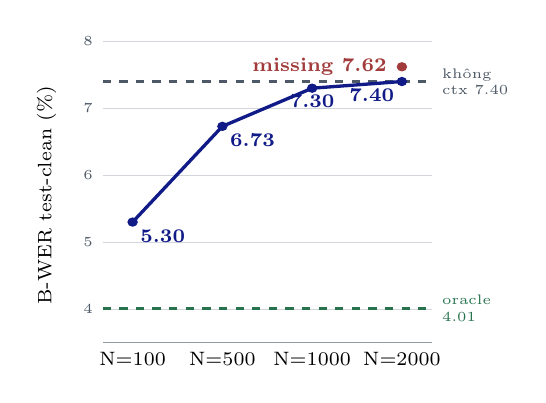
\begin{tikzpicture}[x=0.95cm,y=0.85cm]
\foreach \y in {4,5,6,7,8}{\draw[TextGray!25] (0,\y-3.5)--(4.4,\y-3.5); \node[left,font=\tiny,TextGray] at (0,\y-3.5){\y};}
\draw[TextGray!60] (0,0)--(4.4,0);
\draw[TextGray,dashed,thick] (0,7.40-3.5)--(4.4,7.40-3.5) node[right,font=\tiny,text=TextGray,align=left]{không\\ctx 7.40};
\draw[GoodGreen,dashed,thick] (0,4.01-3.5)--(4.4,4.01-3.5) node[right,font=\tiny,text=GoodGreen,align=left]{oracle\\4.01};
\draw[Primary,very thick] (0.4,5.30-3.5)--(1.6,6.73-3.5)--(2.8,7.30-3.5)--(4.0,7.40-3.5);
\foreach \x/\v/\l/\p in {0.4/5.30/100/below right, 1.6/6.73/500/below right, 2.8/7.30/1000/below, 4.0/7.40/2000/below left}{
  \fill[Primary] (\x,\v-3.5) circle (0.07);
  \node[\p=-1pt,font=\scriptsize\bfseries,text=Primary] at (\x,\v-3.5){\v};
  \node[below,font=\scriptsize] at (\x,0){N=\l};
}
\fill[RiskRed] (4.0,7.62-3.5) circle (0.07) node[left=2pt,font=\scriptsize\bfseries,text=RiskRed]{missing 7.62};
\node[rotate=90,font=\scriptsize] at (-0.75,2.2){B-WER test-clean (\%)};
\end{tikzpicture}
\end{center}
\column{0.56\textwidth}
\scriptsize\renewcommand{\arraystretch}{1.15}\setlength{\tabcolsep}{3pt}
\begin{tabular}{@{}lccc@{}}
\toprule
\textbf{clean / other} & \textbf{WER} & \textbf{U-WER} & \textbf{B-WER}\\
\midrule
Không context & 1.63 / 3.41 & 0.89 / 1.91 & 7.40 / 16.08\\
Oracle & 1.22 / 2.43 & 0.87 / 1.80 & \good{4.01 / 7.73}\\
N=100 & 1.42 / 3.17 & 0.93 / 2.17 & 5.30 / 11.61\\
N=500 & 1.60 / 3.33 & 0.94 / 1.96 & 6.73 / 14.88\\
N=1000 & 1.67 / 3.45 & 0.95 / 1.98 & 7.30 / 15.92\\
N=2000 & 1.69 / 3.55 & 0.96 / 2.02 & \bad{7.40 / 16.45}\\
Missing & 1.73 / 3.50 & 0.98 / 1.98 & \bad{7.62 / 16.34}\\
\bottomrule
\end{tabular}
\end{columns}
\vfill\src{Context = system prompt ``w1, w2, …''; chuẩn hoá Whisper; full test-clean 2620 / test-other 2939 câu}
\end{frame}

\begin{frame}{Số liệu nói lên 3 điều}
\begin{columns}[T,onlytextwidth]
\column{0.32\textwidth}
\begin{block}{1. Context có ích lớn}
\small Oracle: B-WER \textbf{7.40 $\rightarrow$ 4.01} ($-46\%$), U-WER gần như giữ nguyên.\\[3pt]
$\Rightarrow$ Không cần train ASR, chỉ cần \textbf{đưa đúng từ}.
\end{block}
\column{0.32\textwidth}
\begin{alertblock}{2. List dài thì vô dụng}
\small N=100 $\rightarrow$ 2000: B-WER \textbf{5.30 $\rightarrow$ 7.40}, bằng không context.\\[3pt]
Test-other N=2000: \bad{16.45} $>$ 16.08.
\end{alertblock}
\column{0.32\textwidth}
\begin{alertblock}{3. List sai thì có hại}
\small Missing: \bad{7.62} $>$ 7.40 (clean), \bad{16.34} $>$ 16.08 (other).\\[3pt]
$\Rightarrow$ Đưa bừa từ vào prompt là \textbf{phản tác dụng}.
\end{alertblock}
\end{columns}
\vspace{0.4cm}
\begin{beamercolorbox}[sep=0.55em,center,rounded=true]{block body alerted}
\textbf{Điều kiện để hưởng lợi:} list phải \textbf{ngắn} và \textbf{có từ đúng}.\\
\small Khoảng trống cần lấy lại: 7.40 (không context) $\rightarrow$ 4.01 (oracle) $=$ \textbf{3.4 điểm B-WER}.
\end{beamercolorbox}
\end{frame}

% =====================================================================
\section{3. Hướng đi}
\begin{frame}{Paper hiện tại đã giải phần nào? Còn chừa gì?}
\small\renewcommand{\arraystretch}{1.2}
\begin{tabular}{@{}p{2.3cm}p{5.0cm}p{5.0cm}@{}}
\toprule
& \textbf{Hou25} (Interspeech 2025) & \textbf{PTC-Bias} (arXiv 2609.28727)\\
\midrule
Cách làm & Chấm điểm từng từ (TTS audio $\leftrightarrow$ speech) $\rightarrow$ top-50 vào prompt & So phoneme theo thời gian $\rightarrow$ shortlist $\le$10 từ + sửa sau decode\\
Train & scorer & model phoneme\\
Bias list & \bad{cho sẵn, luôn có từ đúng} & \bad{cho sẵn, luôn có từ đúng}\\
Kết quả & Whisper, N=100: B-WER 7.8 $\rightarrow$ 5.4 & \hi{Qwen3-ASR}, N=2000: B-WER \textbf{4.10 / 7.76}\\
\bottomrule
\end{tabular}
\vspace{0.3cm}
\begin{columns}[T,onlytextwidth]
\column{0.48\textwidth}
\begin{block}{Đọc số}
\small PTC-Bias 4.10 / 7.76 $\approx$ oracle của nhóm 4.01 / 7.73\\
$\Rightarrow$ bài \textbf{``chọn từ trong list cho sẵn''} gần như \textbf{đã kịch trần}.
\end{block}
\column{0.48\textwidth}
\begin{alertblock}{Chỗ còn trống}
\small Thực tế \textbf{không có list}. Đã có bài tự tìm context từ \textbf{segment trước} (RAG, EMNLP'25, chỉ đo WER); chưa thấy bài cho \textbf{từng câu, không lịch sử}, trên speech LLM frozen, đo B-WER.
\end{alertblock}
\end{columns}
\vfill\src{Số PTC-Bias trích từ paper (pipeline của họ); oracle là số nhóm tự chạy --- chỉ so sánh tương đối.}
\end{frame}

\begin{frame}{Hướng em đề xuất (chưa chốt method)}
\begin{center}
\begin{tikzpicture}[node distance=0.35cm]
\node[nbox,minimum width=2.0cm,text width=1.9cm] (t) {Topic\\\footnotesize hoặc decode lần 1};
\node[lgbox,right=of t,minimum width=2.2cm,text width=2.1cm] (g) {\textbf{LLM sinh list}\\\footnotesize candidate};
\node[lgbox,right=of g,minimum width=2.4cm,text width=2.3cm] (loc) {\textbf{Tìm chỗ cần nghe kỹ}\\\footnotesize token ASR không chắc};
\node[box,right=of loc,minimum width=2.2cm,text width=2.1cm] (fix) {Can thiệp\\\footnotesize context / logit, ASR frozen};
\draw[arr] (t)--(g); \draw[arr] (g)--(loc); \draw[arr] (loc)--(fix);
\node[below=0.3cm of g,font=\footnotesize\bfseries,text=Accent!70!black] {Giả định H1};
\node[below=0.3cm of loc,font=\footnotesize\bfseries,text=Accent!70!black] {Giả định H2};
\end{tikzpicture}
\end{center}
\vspace{0.1cm}
\begin{columns}[T,onlytextwidth]
\column{0.48\textwidth}
\begin{alertblock}{H1: list tự sinh có chứa từ đúng?}
\small Nếu LLM không đoán ra từ hiếm thì cả hướng sụp $\rightarrow$ phải kiểm \textbf{đầu tiên}.\\
Phương án dự phòng: retrieve từ kho 209k (hướng 1 buổi 17/09).
\end{alertblock}
\column{0.48\textwidth}
\begin{alertblock}{H2: từ sai nằm ở chỗ ASR không chắc?}
\small Nếu đúng $\rightarrow$ chỉ can thiệp ở đó, giữ được U-WER (tránh lỗi ``list sai có hại'' ở trên).
\end{alertblock}
\end{columns}
\vfill\src{Định vị theo thời gian đã có ở PTC-Bias $\Rightarrow$ novelty nằm ở ``không cần list cho sẵn''.}
\end{frame}

% =====================================================================
\section{4. Kế hoạch}
\begin{frame}{2 tuần tới: kiểm H1, H2 trước khi xây method}
\footnotesize\renewcommand{\arraystretch}{1.3}
\begin{tabular}{@{}p{0.4cm}p{4.1cm}p{3.6cm}p{4.3cm}@{}}
\toprule
& \textbf{Thí nghiệm} & \textbf{Đo} & \textbf{Nếu kết quả xấu}\\
\midrule
\hi{1} & LLM sinh $\le$100 từ từ tên sách/chương, hoặc từ bản decode lần 1 & \textbf{Recall@K} so với từ hiếm đúng & Chuyển sang retrieve từ kho 209k\\
\hi{2} & Đưa list đó vào Qwen3-ASR & B-WER so với 7.40 (không ctx) và 5.30 (N=100) & Cần thêm bước lọc/xếp hạng\\
\hi{3} & Log-prob lần decode 1 có ``bắt'' được vị trí từ hiếm sai không & precision / recall theo vị trí & Bỏ H2, can thiệp cả câu\\
\hi{4} & Song song: chạy code PTC-Bias trên pipeline nhóm & có ra 4.10 / 7.76? & Liên hệ tác giả / kiểm setting\\
\bottomrule
\end{tabular}
\vspace{0.3cm}
\begin{beamercolorbox}[sep=0.5em,center,rounded=true]{block body alerted}
\small Cuối 2 tuần (\textbf{$\sim$17/10}) có 4 con số $\Rightarrow$ biết hướng có \textbf{khả thi} không $\Rightarrow$ chốt method với thầy.\\
Tune trên tập dev riêng, không tune trên test.
\end{beamercolorbox}
\end{frame}

\begin{frame}{Lộ trình tới hạn Interspeech 2027 (09/02/2027)}
\begin{center}
\begin{tikzpicture}[x=1.3cm]
\draw[arr,very thick] (0,0)--(10.4,0);
\foreach \x/\pa/\pb/\pc in {
 0.4/{10}/{Feasibility}/{H1, H2\\PTC-Bias},
 2.6/{10--11}/{Chốt \& xây method}/{dev split\\ConEC},
 4.8/{11--12}/{Thí nghiệm chính}/{so Hou25, PTC-Bias\\5 điều kiện},
 7.0/{12--01}/{Ablation}/{phân tích lỗi\\over-biasing},
 9.2/{01--02}/{Viết \& nộp}/{4 trang\\09/02/2027}}{
  \fill[Primary] (\x,0) circle (0.11);
  \node[above=0.15cm,font=\footnotesize\bfseries,text=Primary,align=center] at (\x,0){Tháng \pa\\\pb};
  \node[below=0.2cm,font=\scriptsize,align=center,text=TextGray] at (\x,0){\pc};
}
\end{tikzpicture}
\end{center}
\vspace{0.3cm}
\begin{alertblock}{Mốc kiểm soát}
\small \textbf{17/10}: có số feasibility --- đi tiếp hay đổi hướng. \quad \textbf{Cuối 11}: method thắng baseline ở ít nhất 1 điều kiện khó.
\end{alertblock}
\end{frame}

\begin{frame}{Cần thầy quyết để đi tiếp}
\renewcommand{\arraystretch}{1.35}
\begin{tabular}{@{}cp{7.4cm}p{4.6cm}@{}}
\toprule
& \textbf{Câu hỏi} & \textbf{Đề xuất của nhóm}\\
\midrule
\hi{1} & Chọn bài toán \textbf{``không có list cho sẵn''} làm novelty chính? & Đồng ý --- phần ``chọn'' đã kịch trần\\
\hi{2} & LLM sinh list: chạy \textbf{local} hay gọi \textbf{API}? & Local (vd.\ Qwen3-8B) để tái lập được\\
\hi{3} & Hou25: \textbf{tự implement} (phải train) hay chỉ \textbf{trích số} từ paper? & Trích số trước, implement nếu reviewer cần\\
\hi{4} & Bộ domain thật dùng \textbf{ConEC} (Earnings-21/22)? & Đồng ý ConEC\\
\hi{5} & Dùng lâu dài \textbf{1$\times$RTX 4090} trên server? & Đủ cho toàn bộ kế hoạch\\
\bottomrule
\end{tabular}
\end{frame}

% =====================================================================
\section{Phụ lục}
\begin{frame}{Phụ lục: chọn dataset}
\small\renewcommand{\arraystretch}{1.2}
\begin{tabular}{@{}p{3.4cm}p{1.6cm}p{1.6cm}p{5.6cm}@{}}
\toprule
\textbf{Bộ} & \textbf{Ngôn ngữ} & \textbf{Speech} & \textbf{Quyết định} \\
\midrule
\hi{LibriSpeech + IS21} & EN & thật & \cmark{} \textbf{Chính} --- 5.559 câu test, kho 209.291 từ hiếm (từ dữ liệu train) \\
\hi{ConEC} (Earnings-21/22) & EN & thật & \cmark{} \textbf{Domain} --- context thật: slide, press release, người dự \\
ContextASR-Bench & EN/ZH & TTS & \pmark{} Phụ --- có nhãn domain, nhiều entity \\
thuhcsi/Contextual-Biasing & \bad{ZH} & thật & \xmark{} Từ WenetSpeech; lệch ``làm tiếng Anh trước'' \\
ProfASR-Bench & EN & \bad{TTS} & \xmark{} Chỉ tham khảo \\
Contextual Earnings-22 & EN & thật & \xmark{} Chưa public (``upon acceptance'') \\
\bottomrule
\end{tabular}
\vfill\src{fbai-speech/is21\_deep\_bias; github.com/huangruizhe/ConEC; MrSupW/ContextASR-Bench; github.com/thuhcsi/Contextual-Biasing-Dataset}
\end{frame}

\begin{frame}{Phụ lục: setup chạy và số Whisper}
\small
\begin{columns}[T,onlytextwidth]
\column{0.48\textwidth}
\begin{block}{Cấu hình}
\begin{itemize}\itemsep2pt
\item 1$\times$RTX 4090, image \texttt{nvcr.io/nvidia/pytorch:26.08}.
\item Whisper-large-v3-turbo (HF, greedy), prompt ``naive'', cắt 223 token cuối.
\item Qwen3-ASR-1.7B (\texttt{qwen-asr} 0.0.6), \texttt{context} = system prompt.
\item Code: \texttt{bench/} (build\_is21, run\_*, score, eval\_retrieval).
\end{itemize}
\end{block}
\column{0.48\textwidth}
\begin{block}{Whisper-turbo (clean / other)}
\footnotesize\renewcommand{\arraystretch}{1.15}
\begin{tabular}{@{}lcc@{}}
\toprule
\textbf{plain} & WER & B-WER\\
\midrule
không prompt & 2.64 / 4.87 & 9.43 / 18.92\\
N=100 & 2.55 / 4.20 & 8.04 / 13.98\\
N=2000 & 2.79 / 4.97 & 9.15 / 18.69\\
\midrule
\textbf{Hou25} & & \\
không prompt & 3.2 / 5.3 & 10.4 / 19.7\\
N=100 & 2.7 / 4.8 & 7.8 / 15.2\\
N=2000 & 2.9 / 5.2 & 9.8 / 19.5\\
\bottomrule
\end{tabular}
\end{block}
\end{columns}
\vfill\src{Hou et al., Interspeech 2025, Bảng 1}
\end{frame}

\end{document}
